\documentclass{report}

\usepackage[utf8]{inputenc}
\usepackage[english, russian]{babel}
\usepackage{amssymb, amsfonts, amsmath, color, enumerate, indentfirst, geometry, listings}
\usepackage[pdftex]{graphicx} 

\geometry{a4paper, left=2cm, right=2cm, top=2cm, bottom=2cm}
\definecolor{darkgreen}{rgb}{0.0, 0.5, 0.0}
\lstset{
	language=C++,
	basicstyle=\footnotesize,
	numbers=left,
	numberstyle=\tiny,
	numberfirstline=true,
	numbersep=5pt,
	keywordstyle=\color{blue}\bfseries,
	commentstyle=\color{darkgreen},
	stringstyle=\color{red},
	showspaces=false,
	showstringspaces=false,
	captionpos=t,
	breaklines=true,
	breakatwhitespace=false,
	extendedchars=true,
	frame=tb,
	title=\lstname,
}

\begin{document}
	
\begin{titlepage}
	
	\begin{center}
		\LargeМинистерство науки и высшего образования Российской Федерации\\[\baselineskip]
		Федеральное государственное автономное образовательное\\
		учреждение высшего образования \\
		Национальный исследовательский Нижегородский государственный\\
		университет им. Н.И. Лобачевского\\[\baselineskip]
		Институт информационных технологий, математики и механики \\
	\end{center}
	
	\vspace{4em}
	
	\begin{center}
		\textbf{\LARGEОтчет по лабораторной работе} \\
	\end{center}

	\begin{center}
		\textbf{\LARGE«Умножение разреженных матриц, хранящихся в столбцовом формате»} \\
	\end{center}
	
	\vspace{10em}
	
	\hfill\parbox{6cm}{
		\hspace*{5cm}\hspace*{-5cm}\textbf{Выполнил:} \\ студент группы 381708-1 \\ Ямщиков И.С. \\
		\\
		\hspace*{5cm}\hspace*{-5cm}\textbf{Проверил:}\\ доцент кафедры МОСТ, к.т.н., \\ Сысоев А. В.
	}
	
	\vspace{\fill}
	
	\begin{center} 
		Нижний Новгород \\ 2020 
	\end{center}
	
\end{titlepage}

\setcounter{page}{2}

\tableofcontents
\newpage

\section*{Введение}
\addcontentsline{toc}{section}{Введение}
\par При постановке и решении различных задач возникает потребность в использовании так называемых разреженных матриц. Необходимость в применении такого рода  математических объектов появляется, например, в задачах оптимизации, в решении дифференциальных уравнений в частных производных, в теории графов. Как правило, методы хранения и алгоритмы обработки разреженных матриц существенно усложнены вследствие учета разреженной структуры. В этом случае многие алгоритмы являются более трудоемкими в сравнении с методами обработки обычных матриц. Следовательно, важно уметь применять эффективные методы хранения и обработки разреженных матриц.
\newpage

\section*{Постановка задачи}
\addcontentsline{toc}{section}{Постановка задачи}
\par Требуется реализовать последовательный и параллельные варианты алгоритма умножения разреженных матриц, хранящихся в столбцовом формате. Также необходимо оценить и сравнить эффективность их работы в зависимости от различных входных данных и параметров.
\par Параллельные варианты алгоритма должны быть реализованы с применением:
\begin{itemize}
	\item OpenMP;
	\item TBB;
	\item std::thread.
\end{itemize}
\newpage

\section*{Описание алгоритма}
\addcontentsline{toc}{section}{Описание алгоритма}
\par В общем случае матрица называется разреженной, если  процент ее ненулевых элементов мал. Пусть m - число строк, а n - число столбцов матрицы. NZ - количество ее ненулевых элементов. В данной работе будут использованы матрицы, для которых выполняется равенство $NZ = \sqrt{m*n}$. Сами элементы — вещественные числа (в программной реализации будут использоваться числа типа double).
\par Используемый в данной работе формат хранения матриц — столбцовый. Широко известен как CCS (Compressed Column Storage), в котором подразумевается хранение только ненулевых элементов. Характерные особенности данного формата заключаются в следующем:
\begin{itemize}
	\item матрица хранится в виде трех массивов:
	\begin{itemize}
		\item массив значений ненулевых элементов Value, которые в матрице располагаются построчно, сверху вниз;
		\item массив номеров строк Row;
		\item массив индексов начала столбцов ColIndex;
	\end{itemize}
	\item j-ый элемент в ColIndex указывает на начало j-го столбца;
	\item j-ый столбец в массиве Value располагается в диапазоне от ColIndex[j] до (ColIndex[j + 1] – 1) включительно. Столбец j является нулевым, если выполняется равенство ColIndex[j] = ColIndex[j + 1];
	\item удобный доступ и навигация по столбцам матрицы.
\end{itemize}
\par Пусть A и B — матрицы в формате CCS размерностей $(m_{1}, n_{1})$ и $(m_{2}, n_{2})$ соответственно. Напомним, что умножение двух матриц A и B возможно только при выполнении условия $n_{1} = m_{2}$. Если данное условие выполняется, то результатом матричного умножения является C = A * B, где C — матрица, которая хранится в формате CCS размерности $(m_{1}, n_{2})$. Алгоритм умножения двух разреженных матриц, хранящихся в столбцовом формате, заключается выполнении следующих действий:
\begin{itemize}
	\item инициализация структуры данных для результирующей матрицы C;
	\item транспонирование матрицы A (нахождение $A^{T}$);
	\item последовательное перемножение каждого столбца матрицы B на каждый из столбцов матрицы $A^{T}$ и запись в результирующую матрицу C полученных результатов.
\end{itemize}
\newpage

\section*{Описание схемы распараллеливания}
\addcontentsline{toc}{section}{Описание схемы распараллеливания}
\par Описанная далее схема распараллеливания предназначена для использования в системах с общей памятью.
\par Из описания работы алгоритма видно, что одной из самых трудоемких операций в процессе работы является перемножение столбца одной матрицы на все столбцы другой матрицы. То есть, в процессе вычислений перебираются столбцы матрицы B, после чего дальнейшая работа с ними происходит независимо. Следовательно, удобнее всего организовать параллелизм путем распределения столбцов матрицы B по потокам. То есть, каждый поток работает только с  некоторыми столбцами матрицы B, производя с ними необходимые вычисления. 
\par Согласно описанию алгоритма, необходима последовательная запись результатов в результирующую матрицу C. Однако, потоки могут помешать друг другу сделать это корректно. Для исключения такой ситуации применение механизмов синхронизации приведет лишь к существенным накладным расходам, что отрицательно скажется на эффективности алгоритма. В связи с этим, в данной работе в каждом потоке создаются два локальных рабочих буфера, куда записываются частичные результаты для массивов Value, Row матрицы C. 
\par Отметим, что в ходе вычислений синхронизация записи в массив ColIndex не требуется, так как в процессе работы каждый поток обращается только к "своей"\ части массива, что говорит о том, что доступ к ColIndex осуществляется независимо.
\par После завершения вычислений каждым из потоков все локальные данные по каждому столбцу обрабатываются одним главным потоком, который формирует результат и записывает его в результирующую матрицу C.
\par Схематично вышеописанную схему можно представить следующим образом:
 \begin{figure}[htbp]
	\centering
	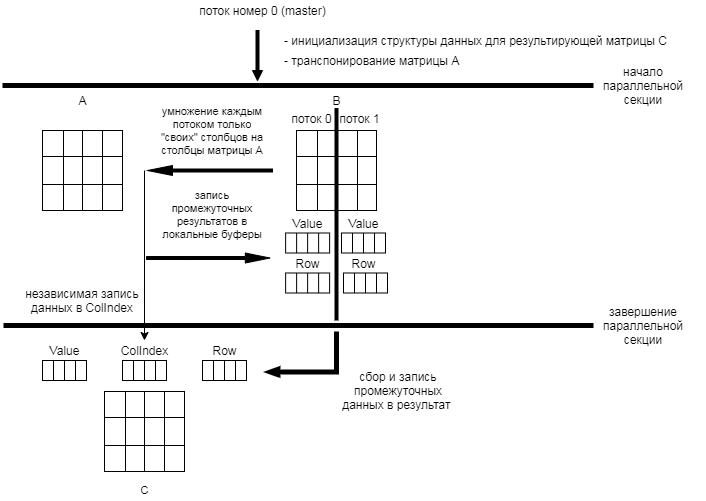
\includegraphics[width=1\textwidth]{parallel_scheme.png}
\end{figure}
\newpage

\section*{Описание программной реализации}
\addcontentsline{toc}{section}{Описание программной реализации}
\par Для хранения матрицы в формате CCS использована структура CcsMatrix со следующими основными полями:
\begin{itemize}
	\item int M — количество строк матрицы;
	\item int N — количество столбцов матрицы;
	\item int not\_zero\_nubers — количество ненулевых элементов матрицы;
	\item vector<double> value — массив значений Value;
	\item vector<int> row — массив Row;
	\item vector<int> colIndex — массив ColIndex.
\end{itemize}
\par В каждой версии алгоритма присутствуют следующие методы:
\begin{itemize}
	\item transposeMatrix — метод, который транспонирует матрицу. На вход поступает константный указатель на матрицу, которую требуется транспонировать. Результат работы метода — объект типа CcsMatrix. Реализация метода одинакова для всех версий алгоритма;
	\item scalarMultiplication — метод, в котором реализовано скалярное умножение двух столбцов матрицы. Входные параметры — константные указатели на матрицы и индексы столбцов, которые требуется перемножить. Результатом работы данной функции является число типа double. Реализация метода одинакова для всех версий алгоритма;
	\item matrixMultiplicate — метод, в котором реализовано непосредственно умножение двух матриц. Последовательность выполняемых действий описана в разделе "Описание алгоритма". Результатом работы метода является объект типа CcsMatrix. Реализация метода разная для каждой версии алгоритма, особенности каждой из них приведены ниже.
\end{itemize}

\subsection*{Последовательная версия}
\addcontentsline{toc}{subsection}{Последовательная версия}
\par Данная версия реализована строго в соответствии с описанием алгоритма. Все действия выполняются последовательно одним потоком. Параллелизм отсутствует. Дополнительной памяти для промежуточных результатов не требуется.

\subsection*{OpenMP-версия}
\addcontentsline{toc}{subsection}{OpenMP-версия}
\par Данная версия реализована в соответствии с описанием алгоритма и схемой распараллеливания. Организация параллельной секции осуществляется при помощи директивы \#pragma omp parallel. В начале параллельной секции в каждом потоке создаются локальные буферы local\_value и local\_row, куда записываются промежуточные результаты в процессе вычислений. Распределение столбцов матрицы B по потокам организовано путем распараллеливания цикла for при помощи директивы \#pragma omp for schedule (static). Завершение цикла автоматически синхронизируется, после чего основной поток master обрабатывает промежуточные данные, записывает их в ColIndex и выделяет память для массивов Value и Row результирующей матрицы C. Далее следует директива \#pragma omp barrier для синхронизации потоков, так как по умолчанию секция master не синхронизируется. После этого каждый поток записывает промежуточные данные из своих локальных буферов в массивы результирующей матрицы, после чего происходит завершение работы параллельной области.

\subsection*{TBB-версия}
\addcontentsline{toc}{subsection}{TBB-версия}
\par Данная версия реализована в соответствии с описанием алгоритма и схемой распараллеливания. В начале главный поток выделяет память под массивы value и row, куда остальные потоки будут записывать промежуточные результаты. Распределение столбцов матрицы B по потокам организовано путем распараллеливания цикла for при помощи функции parallel\_for. Первым аргументом передается одномерное итерационное пространство blocked\_range c параметром grainsize, равным 10. Вторым аргументом передается функтор, в котором реализовано частичное перемножение двух матриц, которое выполняется каждым потоком. После завершения цикла основной поток master обрабатывает промежуточные данные, записывает их в ColIndex и выделяет память для массивов Value и Row результирующей матрицы C. Далее основной поток записывает промежуточные данные из буферов value и row в массивы результирующей матрицы.

\subsection*{std::thread-версия}
\addcontentsline{toc}{subsection}{std::thread-версия}
\par В отличии от предыдущих версий, в текущей реализации отсутствует автоматическое распределение работы по потокам. В связи с чем реализованы следующие функции:
\begin{itemize}
	\item getInvolvedThreadNumber — метод, возвращающий число, равное числу потоков, которое будет выполняться в параллельной секции;
	\item setNumberOfColumn — метод, устанавливающий число столбцов, которое будет обработано каждым потоком;
	\item multOnThread — метод,  в котором реализовано частичное перемножение двух матриц, которое выполняется каждым потоком.
\end{itemize}
\par В начале главный поток выделяет память под массивы value и row, куда остальные потоки будут записывать промежуточные результаты. Далее устанавливается число потоков, которое будет задействовано в параллельной области, а также число столбцов, которое будет обработано каждым потоком. Распределение столбцов матрицы B по потокам организовано в цикле по числу задействованных потоков. То есть, каждый поток в этот момент начинает обработку своих столбцов. Далее основной поток ждет завершения работы других потоков, после чего обрабатывает промежуточные данные, записывает их в ColIndex и выделяет память для массивов Value и Row результирующей матрицы C. Затем основной поток записывает промежуточные данные из буферов value и row в массивы результирующей матрицы.
\newpage

\section*{Результаты экспериментов}
\addcontentsline{toc}{section}{Результаты экспериментов}
\par Характеристики системы:
\begin{itemize}
	\item процессор AMD A4-3300M APU 1.90 GHz;
	\item оперативная память 6 GB;
	\item операционная система Windows 7;
	\item количество ядер 2.
\end{itemize}
\par Эксперименты заключаются в замере времени выполнения умножения двух разреженных матриц. Для удобства используются квадратные матрицы. Входные данные — случайно сгенерированные матрицы порядка N. Замер времени осуществляется при помощи библиотеки chrono. Результаты экспериментов представлены в таблицах ниже:
\begin{table}[htbp]
	\centering
	\begin{tabular}{|c|c|c|c|c|} \hline 
		Версия & Последовательная & OpenMP & TBB & std::thread \\ \hline 
		Порядок матрицы & \multicolumn{4}{|c|}{время, миллисекунд} \\ \hline 
		500 & 4 & 22 & 6 & 8 \\ \hline 
		1000 & 18 & 42 & 21 & 22 \\ \hline 
		5000 & 437 & 271 & 244 & 268 \\ \hline 
		10000 & 1743 & 1071 & 930 & 1003 \\ \hline 
		25000 & 10934 & 6184 & 5581 & 6247 \\ \hline 
		40000 & 28220 & 15581 & 14611 & 15839 \\ \hline 
	\end{tabular}
	\caption{Время выполнения}
\end{table}

\begin{table}[htbp]
	\centering
	\begin{tabular}{|c|c|c|c|} \hline 
		Версия & OpenMP & TBB & std::thread \\ \hline 
		Порядок матрицы & \multicolumn{3}{|c|}{ускорение} \\ \hline 
		500 & 0,18 & 0,66 & 0,5 \\ \hline 
		1000 & 0,43 & 0,86 & 0,82 \\ \hline 
		5000 & 1,61 & 1,79 & 1,63 \\ \hline 
		10000 & 1,63 & 1,87 & 1,74 \\ \hline 
		25000 & 1,77 & 1,96 & 1,75 \\ \hline 
		40000 & 1,81 & 1,93 & 1,78 \\ \hline 
	\end{tabular}
	\caption{Коэффициент ускорения}
\end{table}
\newpage

\section*{Описание подтверждения корректности}
\addcontentsline{toc}{section}{Описание подтверждения корректности}
\par В данной работе помимо самих алгоритмов реализованы unit тесты с использованием GoogleTest для проверки корректности работы методов. Тестируются следующие ситуации:
\begin{itemize}
	\item корректное создание матрицы;
	\item умножение вектора на вектор;
	\item умножение матрицы на вектор;
	\item умножение вектора на матрицу;
	\item умножение матрицы на матрицу.
\end{itemize}
\par Данные тесты были реализованы и успешно выполнены для всех четырех версий метода, что в свою очередь подтверждает корректность всех реализованных в данной работе версий алгоритма умножения разреженных матриц, хранящихся в столбцовом формате.
\newpage

\section*{Выводы}
\addcontentsline{toc}{section}{Выводы}
\par Исходя из результатов проведения экспериментов можно сделать следующие выводы:
\begin{itemize}
	\item если объем решаемой задачи сравнительно невелик и она не является трудоемкой, то использование параллельных версий алгоритмов нецелесообразно, так как затраты на создание потоков и организацию параллельных вычислений превышают затраты на решение задачи последовательным методом. В рамках данной работы применение параллельных алгоритмов оправдано, если порядок матрицы $N \ge 5000$;
	\item TBB-версия оказалась эффективнее других параллельных версий. В данной работе это связано с тем, что работа между потоками распределялась динамически, в отличие от других версий, в которых использовалось статическое распределение задач;
	\item при большой нагрузке версия std::thread оказалась менее эффективной. В данной работе это связано с тем, что задачи между потоками не распределялась автоматически. Балансировка нагрузки осуществлялась вручную статически;
	\item если решаемая задача является трудоемкой, то ускорение работы параллельных версий алгоритма относительно близко к числу работающих потоков при вычислениях.
\end{itemize}
\newpage

\section*{Заключение}
\addcontentsline{toc}{section}{Заключение}
\par В рамках данной работы были реализованы последовательный и параллельные версии алгоритмов умножения разреженных матриц, хранящихся в столбцовом формате. Также были проведены эксперименты, оценивающие реализованные методы. Результаты показали, что TBB-версия является эффективнее других реализаций, а ускорение появляется тогда, когда ресурсов на организацию параллелизма тратится не больше, чем на решение задачи в последовательном случае. Корректность реализованных версий алгоритмов подтверждена проведенными тестами.
\newpage

\section*{Литература}
\addcontentsline{toc}{section}{Литература}
\begin{enumerate}
	\item Корняков К.В., Мееров И.Б., Сиднев А.А., Сысоев А.В., Шишков А.В.
	Инструменты параллельного программирования в системах с общей
	памятью. – Учебное пособие / Под ред. проф. В.П. Гергеля. – Н. Новгород: Изд-во Нижегородского госуниверситета, 2010. – 201 с.
	\item Джордж А., Лю Дж. Численное решение больших разреженных систем уравнений. – М.: Мир, 1984.
	\item Писсанецки С. Технология разреженных матриц. — М.: Мир,1988.
\end{enumerate}
\newpage

\section*{Приложение}
\addcontentsline{toc}{section}{Приложение}

\subsubsection*{Последовательная версия}
\addcontentsline{toc}{subsubsection}{Последовательная версия}
\lstinputlisting[language=C++, caption=Последовательная версия. Заголовочный файл]{../../../../modules/task_1/iamshchikov_i_sparse_matrix_mult/sparse_matrix_mult.h}
\lstinputlisting[language=C++, caption=Последовательная версия. Файл с реализацией]{../../../../modules/task_1/iamshchikov_i_sparse_matrix_mult/sparse_matrix_mult.cpp}
\lstinputlisting[language=C++, caption=Последовательная версия. Файл с тестами]{../../../../modules/task_1/iamshchikov_i_sparse_matrix_mult/main.cpp}
\newpage

\subsubsection*{OpenMP-версия}
\addcontentsline{toc}{subsubsection}{OpenMP-версия}
\lstinputlisting[language=C++, caption=Последовательная версия. Заголовочный файл]{../../../../modules/task_2/iamshchikov_i_sparse_matrix_mult/sparse_matrix_mult.h}
\lstinputlisting[language=C++, caption=Последовательная версия. Файл с реализацией]{../../../../modules/task_2/iamshchikov_i_sparse_matrix_mult/sparse_matrix_mult.cpp}
\lstinputlisting[language=C++, caption=Последовательная версия. Файл с тестами]{../../../../modules/task_2/iamshchikov_i_sparse_matrix_mult/main.cpp}
\newpage

\subsubsection*{std::thread-версия}
\addcontentsline{toc}{subsubsection}{std::thread-версия}
\lstinputlisting[language=C++, caption=Последовательная версия. Заголовочный файл]{../../../../modules/task_4/iamshchikov_i_sparse_matrix_mult/sparse_matrix_mult.h}
\lstinputlisting[language=C++, caption=Последовательная версия. Файл с реализацией]{../../../../modules/task_4/iamshchikov_i_sparse_matrix_mult/sparse_matrix_mult.cpp}
\lstinputlisting[language=C++, caption=Последовательная версия. Файл с тестами]{../../../../modules/task_4/iamshchikov_i_sparse_matrix_mult/main.cpp}
\newpage

\end{document}